\documentclass[11pt]{article}

\usepackage{amsmath}
\usepackage{amssymb}
\DeclareMathOperator*{\argmin}{arg\,min}

\usepackage{graphicx}
\usepackage{subcaption}
\graphicspath{ {paper_figures/} }

\begin{document}

\begin{figure}
\begin{subfigure}{0.5\textwidth}
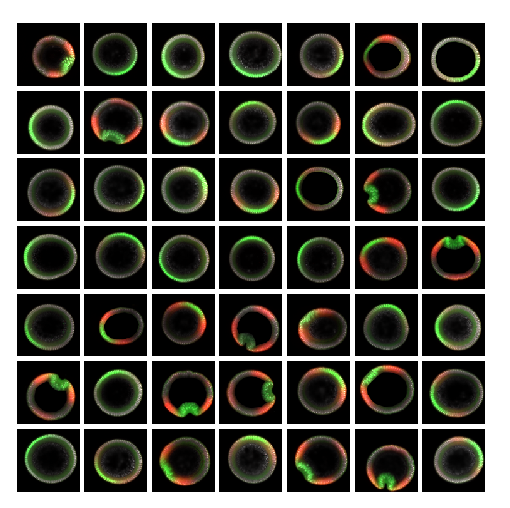
\includegraphics[width=\textwidth]{fig2a}
\caption{}
\end{subfigure}
\begin{subfigure}{0.5\textwidth}
\includegraphics[width=\textwidth]{fig2b}
\caption{}
\end{subfigure}
\caption{} 
\label{fig:fluorescent_images}
\end{figure}

\section{Techniques}

\subsection{Registration Using Angular Synchronization} \label{subsec:angsynch}

Often when one collects images in experiments, each image is taken in a different orientation. 
%
Therefore, the first task in image analysis is to align or {\em register} the set of images. 
%
There are many ways to align images. 
%
``Template--based'' alignment \cite{ahuja2007template} is one technique, where one selects a specific image or {\em template}, and then tries to optimally align each image to that template.
%
However, this method can result in many misalignemnts for noisy images, and can be problematic if a ``good'' template image is not known {\em a priori}. 
%
Instead, we will use a technique called angular synchronization\cite{singer2011angular} to align sets of images.
%
Angular synchronization first computes the pairwise alignments for every possible pair of images, effectively using each image as a template for every other image.
%
From this large collection of pairwise alignments, it then tries to find optimal alignment for each image, such that these individual alignments are most consistent (in some metric) with the pairwise alignment.
%
Because we consider {\em all} pairwise alignments, angular synchronization is often much more robust to noise. 

We will first discuss angular synchronization {\em only} considering rotations. 
%
Let $x_1, \dots, x_m \in \mathbb{R}^x$ denote the signals that we wish to align with respect to rotations.
%
We assume that each signal $x_i$ is a noisy rotated copy of the underlying signal $x_{true}$ (which we are {\em not} given), such that 
\begin{equation}
x_i = f(x_{true}, \theta_i) + \xi_i
\end{equation}
where $f(x_{true}, \theta_i)$ rotates the signal $x_{true}$ by $\theta_i$ degrees, and $\xi_i$ is a noise term (often Gaussian noise). 
%
Our goal is to obtain estimates of $\theta_1, \dots, \theta_m$ so that we can align $x_1, \dots, x_m$. 
%
Up to noise, 
\begin{equation} \label{eq:pairwise_rot}
x_i \approx f(x_j, \theta_i - \theta_j) ;
\end{equation}
 note that \eqref{eq:pairwise_rot} does not require knowledge of $x_{true}$.
%
We can obtain {\em estimates} of $\theta_i - \theta_j$ by computing the rotations to optimally align $x_j$ to $x_i$, 
i.e., $\theta_{ij} \approx \theta_i - \theta_j$, where
%
\begin{equation} \label{eq:opt_angle}
\theta_{ij} = \argmin_{\theta} \|x_i - f(x_j, \theta)\|^2.
\end{equation}

Rather than work with the angles $\theta_{ij}$ directly, it will be more convenient to work with the rotation matrices 
\begin{equation} \label{eq:R_theta}
R(\theta_{ij}) = \begin{bmatrix}
\cos(\theta_{ij}) & \sin(\theta_{ij}) \\
-\sin(\theta_{ij}) & \cos(\theta_{ij})
\end{bmatrix}
\end{equation}
%
Successive rotations correspond to multiplication of the rotation matrices, i.e., 
$R(\alpha_1 + \alpha_2) = R(\alpha_1) R(\alpha_2)$,
and, due to the orthogonality of rotation matrices, $R(-\alpha) = R(\alpha)^T$.

Let $d$ denote the dimension of the rotation matrices we are considering (for our example of planar rotations, $R(\theta_{ij}) \in \mathbb{R}^{2 \times 2}$ and $d=2$; we describe this for general $d$ because we will later consider three--dimensional rotations).
%
We then construct the matrix $H \in \mathbb{R}^{md \times md}$, where $H$ is an $m \times m$ matrix of $d \times d$ blocks with
\begin{equation} \label{eq:H_to_R}
H_{ij} = R(\theta_{ij})
\end{equation}
%

We note that, under our assumption that $\theta_{ij} \approx \theta_i - \theta_j$, 
\begin{equation} 
H_{ij} = R(\theta_{ij}) \approx R(\theta_i - \theta_j) = R(\theta_i) R(-\theta_j) = R(\theta_i) R(\theta_j)^T,
\end{equation}
 and so
\begin{equation} \label{eq:H_low_rank}
	H \approx 
	\begin{bmatrix}
	R(\theta_1) \\
	R(\theta_2) \\
	\vdots \\
	R(\theta_m)
	\end{bmatrix}
	\begin{bmatrix}
	R(\theta_1)^T R(\theta_2)^T \dots R(\theta_m)^T
	\end{bmatrix}
\end{equation}
%
We can (approximately) recover $R(\theta_1), R(\theta_2), \dots, R(\theta_m)$ by computing the top block eigenvector of $H$, which we will denote $\hat{R}$.
%
Let $\phi_1, \phi_2, \dots, \phi_{md}$ denote the eigenvectors of $H$, ordered such that $\lambda_1 \ge \lambda_2 \ge \dots \ge \lambda_{md}$, where $\lambda_i$ is the eigenvalue corresponding to $\phi_i$. 
%
Then
\begin{equation}
\hat{R} = 
\begin{bmatrix}
\hat{R}_1 \\
\hat{R}_2 \\
\vdots \\
\hat{R}_m
\end{bmatrix} =
\begin{bmatrix}
| & | & & | \\
\phi_1 & \phi_2 & \dots & \phi_d \\
| & | & & | 
\end{bmatrix}
\end{equation}
where $\hat{R}_i \in \mathbb{R}^{d \times d}$ is the estimate for $R(\theta_i)$. 
%
Becaus $\hat{R}_i$ is not guaranteed to be a rotation matrix, we project $\hat{R}_i$ onto the closest rotation matrix. 
%
Let $U_i$ and $V_i$ denote the left and right singular vectors, respectively, of $\hat{R}_i$.
%
Then
\begin{equation}
R_{i, est} = U_i V_i^T
\end{equation} 
where $R_{i, est}$ is our estimate of $R(\theta_i)$. 
%
Note that $R_{i, est}$ is not guaranteed to be a proper rotation; because we are permitted to scale the eigenvectors of a matrix, we adjust the sign of $\rho_d$ so that (most of) the rotations are proper. 
%
We can estimate $\theta_{i}$ by inverting \eqref{eq:R_theta}, and then register the signals by rotating image $i$ by $-\theta_i$. 

Furthermore, this eigendecomposition also considers {\em higher--order} consistency information. 
%
For example, given our pairwise estimates $R_{ij}$, we know that relationships of the form
\begin{equation} \label{eq:triplet_consistency}
R(\theta_{ik}) R(\theta_{kj}) \approx R(\theta_i) R(\theta_k)^T R(\theta_k) R(\theta_j)^T = R(\theta_i) R(\theta_j)^T
\end{equation}
should also hold.
%
However, 
\begin{equation}
(H^2)_{ij} = \sum_k R(\theta_{ik}) R(\theta_{kj})
\end{equation}
and so {\em all} infomation of the form in \eqref{eq:triplet_consistency} is contained in the matrix $H^2$.
%
Because $H$ and $H^2$ have the same eigenvectors, our problem formulation accounts for not only pairwise alignment information, but also these higher--order considerations. 

To illustrate how angular synchronization works, we have converted the two--dimensional images into concentration profiles on a ring (we will address the full two--dimensional images in a subsequent section). 
%
Figure \ref{subfig:1d_image_example} shows a typical image that we have converted to a one--dimensional concentration profile. 
%
The images are not aligned, and so rotation of this image corresponds to shifting (with periodic boundary conditions) the one--dimensional concentration profile. 
%
Figure \ref{subfig:1d_unaligned_unordered} shows the concentration profiles for all the images in our data set. 
%
The concentration profiles have been stacked in an array, such that each row corresponds to one image.
%
Figure \ref{subfig:1d_aligned_unordered} shows the concentration profiles, now aligned using angular synchronization. 
%
The peaks are now (mostly) aligned.

\begin{figure}
\begin{subfigure}{0.17\textwidth}
\includegraphics[width=\textwidth]{illustrate_1d}
\caption{}
\label{subfig:1d_image_example}
\end{subfigure}
\begin{subfigure}{0.2\textwidth}
\includegraphics[width=\textwidth]{unregistered_unordered_1d}
\caption{}
\label{subfig:1d_unaligned_unordered}
\end{subfigure}
\begin{subfigure}{0.2\textwidth}
\includegraphics[width=\textwidth]{registered_unordered_1d}
\caption{}
\label{subfig:1d_aligned_unordered}
\end{subfigure}
\begin{subfigure}{0.2\textwidth}
\includegraphics[width=\textwidth]{registered_ordered_1d}
\caption{}
\label{subfig:1d_aligned_ordered}
\end{subfigure}
\begin{subfigure}{0.2\textwidth}
\includegraphics[width=\textwidth]{registered_ordered_vdm_1d}
\caption{}
\label{subfig:1d_aligned_ordered_vdm}
\end{subfigure}
\caption{}
\label{fig:1d_demo}
\end{figure}

\subsection{Ordering Using Diffusion Maps}

Given our set of registered signals, shown in Figure \ref{subfig:1d_aligned_unordered}, we now wish to order them {\em in time} so that we can reconstruct the developmental dynamics.
%
We will use diffusion maps (DMAPS) \cite{coifman2005geometric} to temporally order our data.
%
DMAPS aims to uncover a parameterization of high-dimensional data sampled from a low-dimensional nonlinear manifold.
%
In our framework, we assume that our data lie on a one--dimensional curve or manifold, and that this one dimension is correlated with time. 
%
We will uncover a parameterization of this curve by only considering {\em local} neighbors of each data point.

To illustrate how local neighbors can allow us to uncover a global parameterization, assume we have data $x_1, x_2, \dots, x_m \in \mathbb{R}$ such that $x_1 < x_2 < \dots < x_m$.
%
We consider $x_i$ ``close to'' $x_{i+1}$ and $x_{i-1}$, and $x_i$ ``far away from'' all other data points. 
%
We then construct the (symmetric) weight matrix, $W \in \mathbb{R}^{m \times m}$, where $W_{ij}$ is large if $x_i$ is close to $x_j$,
\begin{equation}
W = 
\begin{bmatrix}
	1 & 1/2 & 0 & 0 & \dots & 0 \\
	1/2 & 1 & 1/2 & 0 & \dots & 0 \\
	\ddots & \ddots & \ddots & \ddots & \ddots & \ddots \\
	0 & 0 & 0 & \dots & 1 & 1/2 \\
	0 & 0 & 0 & \dots & 1/2 & 1 
\end{bmatrix}.
\end{equation}
%
If we normalize this matrix such that $\sum_j W_{ij} = 1$, then one can show that the first eigenvector of this normalized matrix is the all--ones vector, $\phi_1 = [1 1 \dots 1]^T$, and the second eigenvector is a cosine mode, $\phi_2 = [cos(\pi/m) \cos(2 \pi/ m) \dots \cos((m-1) \pi / m) \cos(\pi)]^T$.
%
Therefore, the second eigenvector, $\phi_2$ is {\em one--to--one} with the parameterization of the data, i.e. $\phi_2(1) < \phi_2(2) < \dots < \phi_2(m)$, just as $x_1 < x_2 < \dots < x_m$. 
%
Therefore, sorting our data by the value of the entries in $\phi_2$ will allow us to order our data.

For the above analysis, the key step was having a notion of ``closeness'' between data points so that we can construct the matrix $W$.
%
For general data in high--dimensional space, we typically use a Gaussian kernel to construct $W$,
\begin{equation} \label{eq:dmaps_W}
W_{ij} = \exp \left( -\frac{d^2(x_i, x_j)}{\epsilon^2} \right)
\end{equation}
and $\epsilon$ is a characteristic distance between data points.
%
Therefore, points closer than $\epsilon$ apart are considered ``close'' and points farther than $\epsilon$ apart are considered ``far away''.
%
$\epsilon$ can be chosen using several techniques (see, for example \cite{coifman2008graph}); in practice, we choose $\epsilon$ to be the median of the pairwise distances between data points.

We then compute the diagonal matrix $D$, where $D_{ii} = \sum_{j=1}^{m} W_{ij}$, and the matrix $A$, where
\begin{equation} \label{eq:dmaps_A}
A = D^{-1} W.
\end{equation} 
%
We calculate the eigenvectors $\phi_1, \phi_2, \dots, \phi_m$ and eigenvalues $\lambda_1, \lambda_2, \dots, \lambda_m$ and order them such that $|\lambda_1| \ge |\lambda_2| \ge \dots \ge |\lambda_m|$ \footnote{Because the matrix $A$ is similar to the symmetric matrix $D^{-1/2} W D^{-1/2}$, $A$ is guaranteed to have real eigenvalues and real, orthogonal eigenvectors.}. 
%
Because the matrix $A$ is row-stochastic, $\lambda_1=1$ and $\phi_1$ is a constant vector.
%
In general, the next few eigenvectors $\phi_2, \dots, \phi_m$ give ``meaningful'' embedding coordinates for the data, such that $\phi_j(i)$ gives the $j^{th}$ embedding coordinate of the $i^{th}$ data point. 
%
In our setup, we assume that our data are inherently one--dimensional, and that this one dimension is correlated with time.
%
Therefore, ordering our data by $\phi_2(j)$ will allow us to automatically order our data in time. 

We demonstrate how we can do this with our one--dimensional concentration profiles. 
%
We use the Euclidean distance between the aligned concentration profiles (the rows of Figure \ref{subfig:1d_aligned_unordered}) as our distances in \eqref{eq:dmaps_W}.
%
Figure \ref{subfig:1d_aligned_ordered} shows the data from Figure \ref{subfig:1d_aligned_unordered}, now sorted by the value of the first (non--trivial) dmaps component, $\phi_2$. 

\subsection{Vector Diffusion Maps}

Many times, we would to both align and order our data.
%
Our proposed alignment methodology, angular synchronization, utilizes the eigendecompostion of the matrix $H \in \mathbb{R}^{md \times md}$, and our proposed ordering algorithm, diffusion maps, utilizes the eigendecomposition of the matrix $A \in \mathbb{R}^{m \times m}$.
%
We can combine the two steps into one eigencomputation that allows us to {\em simultaneously} recover the optimal alignments and the temporal ordering.
%
This technique is called vector diffusion maps (VDM) \cite{singer2012vector}.
%
It not only reduces the number of required eigencomputations, but also is much more robust to noise, as mistakes in alignment are also considered when ordering the data.

For vector diffusion maps, we construct the matrix $S \in \mathbb{R}^{md \times md}$, with
\begin{equation}
	S_{ij} = A_{ij} H_{ij}
\end{equation}
%
where $A$ is defined in \eqref{eq:dmaps_A} and $H$ is defined in \eqref{eq:H_to_R}.
%
The distance $d(x_i, x_j)$ used to compute $W_{ij}$ is the distance between samples {\em after} pairwise alignment (i.e. it is the minimium obtained in \eqref{eq:opt_pairwise}). 

We then compute the eigenvalues $\lambda_1, \lambda_2, \dots, \lambda_{md}$ and eigenvectors $\phi_1, \phi_2, \dots, \phi_{md}$ of $S$, and order them such that $|\lambda_1| \ge |\lambda_2| \ge \dots \ge |\lambda_{md}|$.
%
Again, the top (block) eigenvector of $S$ contains approximations of the optimal rotations for each image.
%
However, we now also obtain embedding coordinates for our images.
%
In general, the embedding coordinates are given by 
\begin{equation}
\psi_{k,l} (i) = \langle \phi_k(i), \phi_l(i) \rangle
\end{equation}
where $\phi_k(i) \in \mathbb{R}^d$ denotes the $i^{th}$ block of $\phi_k$.
%
If we assume that our data are one--dimensional, and that the rotations and the dynamics are uncoupled and therefore separable, one can show that a parameterization of our data (i.e. the analog of $\phi_2$ from the diffusion maps case) is given by $\psi_{1,d+1}$.
%
If no such claims can be made, then one often runs a second step of diffusion maps, using $\psi_{k,l}$ as the coordinates, in order to uncover the true manifold modulo symmetries. 

Figure \ref{subfig:1d_aligned_ordered_vdm} shows the result of aligning and ordering the data in Figure \ref{subfig:1d_unaligned_unordered} using vector diffusion maps. 
%
The data has been ordered by $\psi_{1, 3}$. 

\subsection{Registering Images with Respect to Translations and Rotations} \label{subsec:trans_rot_register}

We are not only interested in registering the one--dimensional concentration profiles with respect to rotational symmetries, but we would also like to register the two--dimensional images shown in Figure \ref{fig:fluorescent_images} with respect to rotations {\em and} translations. 
%
However, for \eqref{eq:H_low_rank} to be satisfied, we require that the matrices used to represent the symmetry group be orthogonal, i.e. $R(\alpha)^{-1} = R(\alpha)^T$. 
%
The typical matrix representation for the group of two--dimensional translations and rotations (using the matrix representation for the affine group \cite{...}) does not satisfy this property. 
%
However, we can (approximately) represent rotations and translations in two--dimensions using three--dimensional rotation matrices.
%
We do this by projecting the image onto a portion of the surface of a (three--dimensional) sphere (see Appendix).
%
Rotations in two--dimensions now correspond to rotations around one principal axis in three--dimensions, and translations in two--dimensions correspond (approximately) to rotations around the other two principal axes in three--dimensions \footnote{Clearly, not all translations can be described this way, as translations can range from $-\infty$ to $+ \infty$, and rotations are only from $0$ to $2 \pi$. However, the images we will be considering are already mostly centered, and so we are only interested in small translations that are well within the $[0, 2\pi)$ range.}.
%
These rotation matrices are (by definition) orthoganol, and successive applications of various translations and rotations can be described via multiplication of the corresponding rotation matrices in $SO(3)$.
%
See the Appendix for more details.

\section{Results}

\begin{figure}
\begin{subfigure}{0.5\textwidth}
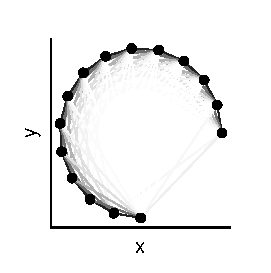
\includegraphics[width=\textwidth]{fig4a}
\caption{}
\end{subfigure}
\begin{subfigure}{0.5\textwidth}
\includegraphics[width=\textwidth]{dpERK_rank_corr}
\caption{}
\end{subfigure}
\begin{subfigure}{0.5\textwidth}
\includegraphics[width=\textwidth]{fig4c}
\caption{}
\end{subfigure}
\begin{subfigure}{0.5\textwidth}
\includegraphics[width=\textwidth]{Dl_rank_corr}
\caption{}
\end{subfigure}
\end{figure}

\appendix

\section{Computing Optimal Alignments for One--Dimensional Signals} 

Each signal shown in Figure \ref{fig:1d_demo} is discretized into 100 points. 
%
To compute the optimal angles in \eqref{eq:opt_angle}, we exhaustively search over all 100 possible shifts/rotations of the signals. 

\section{Computing Optimal Pairwise Alignments for Two--Dimensional Images}

The first step in angular synchronization or vector diffusion maps is to compute the translations and rotations to optimally align each pair of data points. 
%
For each image pair $I_i$ and $I_j$, we solve
\begin{equation}\label{eq:opt_pairwise}
(\theta_{ij}, dx_{ij}, dy_{ij}) = \argmin_{
\begin{matrix}
\theta \in [0, 2\pi) \\ 
dx \in [-\Delta, \Delta]\\ 
dy \in [-\Delta, \Delta]
\end{matrix}
} \|g(I_j, \theta, dx, dy) - I_i \|_F^2.
\end{equation}
where $\| \cdot \|_F$ denotes the Frobenius norm, $\Delta$ is the maximum number of pixels by which we are allowed to translate the image, and $g(I_j, \theta, dx, dy)$ is a function that first rotates the image $I_j$ by $\theta$ degrees, then translates the image by $dx$ pixels in the $x$ direction, and finally translates the image by $dy$ pixels in the $y$ direction. 
%
The image rotation is done with the \texttt{imrotate} function in Matlab, using nearest neighbor interpolation to interpolate the intensities of the pixels (since there is no direct mapping of the pixels of the unrotated image to the pixels of the rotated image).
%
Also, the missing pixels in the rotated image due to corner effects are taken to be black.
%
The translations are done by shifting the pixels with periodic boundary conditions.
%
In \eqref{eq:opt_pairwise}, $\Delta$ is chosen such that only edge pixels with little to no signal are shifted, and the main image is not split or separated when translating (we take $\Delta=20$, which corresponds to a 20\% shift in the image).
%
We only consider shifts that correspond to an integer number of pixels, to remove the need for interpolation when doing the translations.  

The solution to \eqref{eq:opt_pairwise} is not easily computed, as the objective function will most likely be nonconvex.
%
Therefore, instead of using an optimization procedure to compute the solution to \eqref{eq:opt_pairwise}, we choose to discretize the search space and exhaustively search to estimate the solution to \eqref{eq:opt_pairwise}.
%
We discritize the search space of rotations into 20 possible rotations ($d\theta  \in \{0, \pi/10, \pi/5, \dots, 9 \pi/5, 19\pi/10 \}$), and 11 possible translations in both the $x$ and $y$ directions ($dx, dy \in \{-20, -16, -12, \dots, 12, 16, 20 \}$). 
%
We then check all possible combinations for the best rotation and translations that align $I_j$ to $I_i$. 
%
Although this can be somewhat time intensive, it is not prohibitive for the size of data sets which we are considering, and can be trivially parallelized for larger data sets if necessary.
%
The solution to this search will not be the exact solution to \eqref{eq:opt_pairwise}, but it will (most likely) be a close approximation.
%
Since our techniques are robust to noise, close approximations will be sufficient to obtain accurate results.

\section{Converting from $ISO(2)$ to $SO(3)$}

\begin{figure}
\begin{subfigure}{0.2\textwidth}
\includegraphics[width=\textwidth]{sphere_1}
\includegraphics[width=\textwidth]{sphere2_1}
\caption{}
\end{subfigure}
\begin{subfigure}{0.2\textwidth}
\includegraphics[width=\textwidth]{sphere_2}
\includegraphics[width=\textwidth]{sphere2_2}
\caption{}
\end{subfigure}
\begin{subfigure}{0.2\textwidth}
\includegraphics[width=\textwidth]{sphere_3}
\includegraphics[width=\textwidth]{sphere2_3}
\caption{}
\end{subfigure}
\begin{subfigure}{0.2\textwidth}
\includegraphics[width=\textwidth]{sphere_4}
\includegraphics[width=\textwidth]{sphere2_4}
\caption{}
\end{subfigure}
\caption{Illustration of how rotations in three dimensions correspond to translations and rotations in two dimensions. (a) The original image. (b) Rotation around the x--axis (Euler angle $\alpha$) in three dimensions corresponds to rotation of the image. (c) Rotation around the y--axis (Euler angle $\beta$) in three dimensions corresponds to horizontal translation. (d) Rotation around the z--axis (Euler angle $\gamma$) in three dimensions corresponds to vertical translation. The top row shows the three--dimensional spheres, and the bottom row shows the (two--dimensional) surface of the sphere in which we are interested.}
\end{figure}

As discussed in Section \ref{subsec:trans_rot_register}, the underlying symmetry group needs to have a real and orthoganol matrix representation. 
%
We therefore convert $ISO(2)$, the group of two--dimensional translations and rotations, to $SO(3)$, the group of three--dimensional rotations. 
%
In the space of three--dimensional rotations, the Euler angles $\alpha_{ij}$, $\beta_{ij}$, and $\gamma_{ij}$ correspond to
\begin{equation} \label{eq:angle_relations}
\begin{aligned}
	\alpha_{ij} &= \theta_{ij} \\
	\beta_{ij} &= \frac{dx_{ij}}{n} \times \eta_{proj} \\
	\gamma_{ij} &= \frac{dy_{ij}}{n} \times \eta_{proj} \\
\end{aligned}
\end{equation}
where $\eta_{proj}$ is the angular portion of the sphere onto which we choose to project the image.
%
We take $\eta_{proj} =  \pi/8$, so the image lies on a $\pi/8 \times \pi/8$ radians portion of the unit sphere in $\mathbb{R}^3$.
%
From here, we can write rotations around the three principal axes in terms of the three Euler angles
\begin{equation}
\begin{aligned}
	R^x_{ij} &= \begin{bmatrix}
	1 & 0 & 0 \\
    0 & \cos(\alpha) & -\sin(\alpha) \\
    0 & \sin(\alpha) & \cos(\alpha)
	\end{bmatrix} \\
	R^y_{ij} &= \begin{bmatrix}
	\cos(\beta) & 0 & \sin(\beta) \\
    0 & 1 & 0 \\
    -\sin(\beta) & 0 & \cos(\beta)
    \end{bmatrix} \\
	R^z_{ij} &= \begin{bmatrix} 
	\cos(\gamma) & -\sin(\gamma) & 0 \\
    \sin(\gamma) & \cos(\gamma) & 0 \\
    0 & 0 & 1 
    \end{bmatrix}
\end{aligned}
\end{equation}
where $R^x_{ij}$, $R^y_{ij}$, and $R^z_{ij}$ correspond to rotations around the $x$, $y$, and $z$ axes, respectively.
%
We then write the total rotation $R_{ij} \in SO(3)$ as 
\begin{equation} \label{eq:total_rot}
	R_{ij}	 = R^z_{ij} \times R^y_{ij} \times R^x_{ij}
\end{equation}
%
\eqref{eq:total_rot} corresponds to first rotating the image by $\theta$, then translating the image by $dx$ pixels in the $x$ direction, and finally translating the image by $dy$ pixels in the $y$ direction (we note that, because the rotation matrices operate from the left, the rightmost rotation matrix in the product in \eqref{eq:total_rot} corresponds to the first operation we perform on the image).

\section{Computing Optimal Translations and Rotations from the Eigenvectors of $H$}

We then compute the three--dimensional rotation, $R_{ij} \in SO(3)$, from the two--dimensional translation and rotation parameters $\theta_{ij}$, $dx_{ij}$, and $dy_{ij}$ (see Appendix for more details).
%
We then build the matrix $H$ and compute the estimates $R_{i, est}$ as described in Section \ref{subsec:angsynch}.
%
From the matrices $R_{1, opt}, \dots, R_{m, opt}$, we now wish to find the corresponding translations and rotations of the images.
%
Because we are permitted to adjust our rotations by a global rotations, we first multiply all rotations by $R_1^T$ to ensure that all the images are (approximately) in the region of the sphere where we began.
%
We then compute the Euler angles $\alpha$, $\beta$, and $\gamma$ from the rotation matrix $R$ using the following relationships
\begin{equation}
\begin{aligned}
R_{1,1} & = \cos(\beta)\cos(\gamma) \\
R_{2,1} & = \cos(\beta)\sin(\gamma) \\
R_{3,1} & = -\sin(\beta) \\
R_{3,2} & = \sin(\alpha)\cos(\beta) \\
R_{3,3} & = \cos(\alpha)\cos(\beta) 
\end{aligned}
\end{equation}
%
We can then invert \eqref{eq:angle_relations} to compute the optimal translation and rotation for each image from the Euler angles.
%
We round the optimal translations to the nearest integer.

\bibliographystyle{plain}
\bibliography{../../references/references}

\end{document}